\documentclass[aspectratio=169,11pt,t]{beamer}

% ============================================================
% Theme and typography
% ============================================================

\usetheme{Madrid}
\usecolortheme{default}
\usefonttheme{professionalfonts}

\setbeamertemplate{navigation symbols}{}
\setbeamertemplate{headline}{}

\setbeamertemplate{footline}{%
  \leavevmode\hbox{%
  \begin{beamercolorbox}[wd=.82\paperwidth,ht=2.5ex,dp=1.0ex,leftskip=.8em]{author in head/foot}
    CSCI 6461 --- Computer Systems Architecture
  \end{beamercolorbox}%
  \begin{beamercolorbox}[wd=.18\paperwidth,ht=2.5ex,dp=1.0ex,rightskip=.8em]{date in head/foot}
    \hfill\insertframenumber/\inserttotalframenumber
  \end{beamercolorbox}}
}

\setbeamersize{text margin left=0.65cm,text margin right=0.65cm}

\setbeamerfont{frametitle}{size=\Large, series=\bfseries}
\setbeamerfont{block title}{size=\normalsize, series=\bfseries}
\setbeamertemplate{blocks}[rounded][shadow=false]

\addtobeamertemplate{block begin}{\vspace{0.1em}}{\vspace{0.1em}}
\addtobeamertemplate{block end}{}{\vspace{0.2em}}

\setbeamertemplate{itemize/enumerate body begin}{\setlength{\itemsep}{4pt}}
\setbeamertemplate{itemize/enumerate subbody begin}{\setlength{\itemsep}{2pt}}

% ============================================================
% Packages
% ============================================================

\usepackage[T1]{fontenc}
\usepackage{lmodern}
\usepackage{iftex}
\ifPDFTeX
  \usepackage[scale=0.92]{sourcecodepro}
\else
  \usepackage{fontspec}
  \setmonofont{Source Code Pro}[Scale=0.92]
\fi
\usepackage{amsmath}
\usepackage{booktabs}
\usepackage{array}
\usepackage{colortbl}
\usepackage{tikz}
\usepackage{adjustbox}

\usetikzlibrary{arrows.meta,positioning,shapes.geometric,calc,decorations.pathreplacing}

% ============================================================
% Colors
% ============================================================

\definecolor{navy}{RGB}{24,43,68}
\definecolor{deepblue}{RGB}{45,88,130}
\definecolor{lightblue}{RGB}{235,242,250}
\definecolor{softgray}{RGB}{245,247,250}
\definecolor{darkgray}{RGB}{25,28,32}
\definecolor{gold}{RGB}{200,145,35}
\definecolor{softgreen}{RGB}{226,242,232}
\definecolor{softorange}{RGB}{253,238,215}
\definecolor{softpurple}{RGB}{238,234,250}

\setbeamercolor{palette primary}{bg=navy,fg=white}
\setbeamercolor{palette secondary}{bg=deepblue,fg=white}
\setbeamercolor{frametitle}{bg=navy,fg=white}
\setbeamercolor{title}{fg=white}
\setbeamercolor{subtitle}{fg=white}
\setbeamercolor{author}{fg=white}
\setbeamercolor{date}{fg=white}
\setbeamercolor{titlelike}{fg=white}
\setbeamercolor{block title}{bg=deepblue,fg=white}
\setbeamercolor{block body}{bg=lightblue,fg=darkgray}
\setbeamercolor{normal text}{fg=darkgray,bg=white}

% ============================================================
% Formatting shortcuts
% ============================================================

\setlength{\parskip}{0pt}
\newcommand{\key}[1]{\textbf{#1}}
\newcommand{\bits}[1]{\texttt{#1}}
\newcommand{\hex}[1]{\texttt{0x#1}}
\newcommand{\code}[1]{\texttt{#1}}

\newcommand{\bfld}[5]{%
  \pgfmathsetmacro{\cx}{#1 + #3/2}%
  \fill[#5] (#1,#2) rectangle ++(#3,0.72);%
  \draw[navy,line width=0.7pt] (#1,#2) rectangle ++(#3,0.72);%
  \node[font=\ttfamily\scriptsize,align=center,text=darkgray] at (\cx,#2+0.36) {#4};%
}

\newcommand{\sectiondivider}[2]{%
\begin{frame}[plain]
\begin{tikzpicture}[remember picture,overlay]
\fill[navy] (current page.south west) rectangle (current page.north east);
\fill[gold] (current page.south west) rectangle ([yshift=.15cm]current page.south east);
% Explicit page coordinates keep the divider independent of top-aligned frames.
\node[anchor=west,inner sep=0pt,text width=.93\paperwidth] at
  ([xshift=.55cm,yshift=.12\paperheight]current page.west) {%
\raggedright
\hyphenpenalty=10000
\exhyphenpenalty=10000
{\color{gold}\large\bfseries #1\par}
\vspace{0.3cm}
{\color{white}\fontsize{22}{26}\selectfont\bfseries #2\par}
};
\end{tikzpicture}
\end{frame}
}

\tikzset{
  unit/.style={draw=navy,line width=0.8pt,rounded corners=2pt,fill=lightblue,minimum width=2.35cm,minimum height=0.82cm,align=center,font=\small},
  state/.style={unit,fill=gold!24},
  logic/.style={unit,fill=softgreen},
  controlunit/.style={logic,fill=softpurple,draw=deepblue,dash pattern=on 3pt off 2pt},
  arr/.style={-{Stealth[length=2.2mm]},draw=navy,line width=0.8pt},
  bus/.style={-{Stealth[length=2.2mm]},draw=navy,line width=1.0pt},
  ctrl/.style={-{Stealth[length=2.0mm]},draw=deepblue,line width=0.8pt,dashed}
}
\tikzset{
  memblock/.style={state,minimum width=3.15cm,minimum height=1.05cm},
  regblock/.style={state,minimum width=2.35cm,minimum height=1.45cm}
}



% Multiplexers: two data inputs on the base, one output at the tip.
% The dashed selection control meets a sloping edge.
\tikzset{
  pics/muxright/.style args={#1}{code={
    \draw[draw=navy,line width=.9pt,fill=softorange]
      (0,.7)--(0,-.7)--(1.05,0)--cycle;
    \node[font=\ttfamily\scriptsize,align=center,inner sep=0pt] at (.35,0) {#1};
    \coordinate (-upper) at (0,.35);
    \coordinate (-lower) at (0,-.35);
    \coordinate (-out) at (1.05,0);
    \coordinate (-selN) at (.45,.4);
    \coordinate (-selS) at (.45,-.4);
  }},
  pics/muxwriteback/.style={code={
    \draw[draw=navy,line width=.9pt,fill=softorange]
      (0,.8)--(0,-.8)--(1.4,0)--cycle;
    \node[font=\ttfamily\scriptsize,align=center,inner sep=0pt] at (.36,0) {WB\\mux};
    \coordinate (-upper) at (0,.35);
    \coordinate (-lower) at (0,-.35);
    \coordinate (-out) at (1.4,0);
    \coordinate (-selN) at (.5,.514286);
  }},
  pics/muxread2/.style={code={
    \draw[draw=navy,line width=.9pt,fill=softorange]
      (0,.35)--(0,-.35)--(.6,0)--cycle;
    \coordinate (-upper) at (0,.175);
    \coordinate (-lower) at (0,-.175);
    \coordinate (-out) at (.6,0);
    \coordinate (-selN) at (.26,.198333);
    \node[font=\ttfamily\tiny,anchor=west,inner sep=0pt] at (.07,.175) {0};
    \node[font=\ttfamily\tiny,anchor=west,inner sep=0pt] at (.07,-.175) {1};
  }}
}

% Detailed component symbols with explicit pin coordinates.
\tikzset{
  componentbody/.style={draw=black!60,line width=1.1pt,fill=white},
  componentpin/.style={draw=black!60,line width=.9pt},
  pinlabel/.style={font=\ttfamily\small,text=black!65,inner sep=2pt},
  componentlabel/.style={font=\small\bfseries,text=black!65,align=center},
  pics/regfile/.style={code={
    \draw[componentbody] (0,-1.5) rectangle (3.1,1.5);
    \draw[componentpin] (.35,1.5)--(.55,1.25)--(.75,1.5);
    \coordinate (-CLK) at (.55,2.05);
    \coordinate (-WE3) at (1.85,2.05);
    \draw[componentpin] (-CLK)--(.55,1.5);
    \draw[componentpin] (-WE3)--(1.85,1.5);
    \node[pinlabel,above] at (-CLK) {CLK};
    \node[pinlabel,anchor=north] at (1.85,1.45) {WE3};
    \foreach \name/\yy in {A1/1,A2/.25,A3/-.55,WD3/-1.12} {
      \coordinate (-\name) at (-.55,\yy);
      \draw[componentpin] (-\name)--(0,\yy);
      \node[pinlabel,anchor=west] at (.08,\yy) {\name};
    }
    \foreach \name/\yy in {RD1/1,RD2/.25} {
      \coordinate (-\name) at (3.65,\yy);
      \draw[componentpin] (3.1,\yy)--(-\name);
      \node[pinlabel,anchor=east] at (3.02,\yy) {\name};
    }
    \node[componentlabel] at (1.72,-.65) {Register\\File};
  }},
  pics/imem/.style={code={
    \draw[componentbody] (0,-1.1) rectangle (2.5,1.3);
    \coordinate (-A) at (-.55,.5);
    \coordinate (-RD) at (3.05,.5);
    \draw[componentpin] (-A)--(0,.5);
    \draw[componentpin] (2.5,.5)--(-RD);
    \node[pinlabel,anchor=west] at (.08,.5) {A};
    \node[pinlabel,anchor=east] at (2.42,.5) {RD};
    \node[componentlabel] at (1.25,-.25) {Instruction\\Memory};
  }},
  pics/dmem/.style={code={
    \draw[componentbody] (0,-1.5) rectangle (3.1,1.5);
    \draw[componentpin] (.35,1.5)--(.55,1.25)--(.75,1.5);
    \coordinate (-CLK) at (.55,2.05);
    \coordinate (-WE) at (2.1,2.05);
    \draw[componentpin] (-CLK)--(.55,1.5);
    \draw[componentpin] (-WE)--(2.1,1.5);
    \node[pinlabel,above] at (-CLK) {CLK};
    \node[pinlabel,anchor=north] at (2.1,1.45) {WE};
    \coordinate (-A) at (-.55,.85);
    \coordinate (-WD) at (-.55,-1);
    \coordinate (-RD) at (3.65,.85);
    \draw[componentpin] (-A)--(0,.85);
    \draw[componentpin] (-WD)--(0,-1);
    \draw[componentpin] (3.1,.85)--(-RD);
    \node[pinlabel,anchor=west] at (.08,.85) {A};
    \node[pinlabel,anchor=west] at (.08,-1) {WD};
    \node[pinlabel,anchor=east] at (3.02,.85) {RD};
    \node[componentlabel] at (1.7,-.4) {Data\\Memory};
  }},
  pics/alu/.style={code={
    \draw[componentbody] (0,1.4)--(1.3,1)--(1.3,-1)--(0,-1.4)
      --(0,-.35)--(.45,0)--(0,.35)--cycle;
    \coordinate (-SrcA) at (-1.1,.8);
    \coordinate (-SrcB) at (-1.1,-.8);
    \coordinate (-Result) at (2.35,.5);
    \coordinate (-NZCV) at (2.35,-.6);
    \coordinate (-Control) at (.7,1.95);
    \draw[componentpin] (-SrcA)--(0,.8);
    \draw[componentpin] (-SrcB)--(0,-.8);
    \draw[componentpin] (1.3,.5)--(-Result);
    \draw[componentpin] (1.3,-.6)--(-NZCV);
    \draw[componentpin] (-Control)--(.7,1.185);
    \node[pinlabel,above] at (-.55,.8) {SrcA};
    \node[pinlabel,above] at (-.55,-.8) {SrcB};
    \node[pinlabel,above] at (1.98,.5) {Result};
    \node[pinlabel,below] at (1.98,-.6) {NZCV};
    \node[pinlabel,above] at (-Control) {ALUControl};
    \node[componentlabel,rotate=90] at (.92,0) {ALU};
  }},
  pics/immext/.style={code={
    \draw[componentbody] (0,-.25)--(3.3,-.55)--(3.3,.55)--(0,.25)--cycle;
    \coordinate (-Instr) at (-1.15,0);
    \coordinate (-ExtImm) at (4,0);
    \coordinate (-ImmSrc) at (1.9,1.25);
    \draw[componentpin] (-Instr)--(0,0);
    \draw[componentpin] (3.3,0)--(-ExtImm);
    \draw[componentpin] (-ImmSrc)--(1.9,.423);
    \node[pinlabel,above] at (-.6,0) {Instr};
    \node[pinlabel,above] at (3.65,0) {ExtImm};
    \node[pinlabel,above] at (-ImmSrc) {ImmSrc};
    \node[componentlabel] at (1.95,0) {Imm Ext};
    \node[font=\scriptsize,text=black!65] at (-.6,-.55) {32 bits};
    \node[font=\scriptsize,text=black!65] at (3.65,-.8) {64 bits};
  }}
}
% Topic 10 uses the approved Topic 8/9 typography and page geometry.
\newcolumntype{R}[1]{>{\raggedright\arraybackslash}p{#1}}
\newcommand{\Asm}[1]{{\ttfamily\small\begin{tabular}{@{}l@{}}#1\end{tabular}}}
\newcommand{\SourceNote}[1]{\par\vspace{.08cm}{\tiny\color{deepblue}#1\par}}
\newcommand{\Model}[1]{\par{\scriptsize\color{deepblue}\textbf{Example assumptions:} #1\par}\vspace{.14cm}}
\tikzset{
  memcell/.style={draw=navy,line width=.65pt,minimum width=1.22cm,minimum height=.65cm,inner sep=2pt,align=center,font=\scriptsize\ttfamily},
  cachebox/.style={unit,minimum width=2.8cm,minimum height=.78cm},
  twoway/.style={Latex-Latex,draw=navy,line width=.9pt},
  memcross/.style={preaction={draw=white,line width=3pt}}
}
\newcommand{\EightWords}[1]{%
  \foreach \i in {0,...,7} {
    \pgfmathtruncatemacro{\off}{8*\i}
    \node[memcell,fill=#1] (word\i) at ({1.26*\i},0) {\off-\the\numexpr\off+7\relax};
  }
}
\title[Topic 10]{Memory Hierarchy, Locality, \& Cache Fundamentals}
\subtitle{AArch64 memory accesses, cache organization, write policies, and performance}
\author{Computer Systems Architecture}
\date{}
\begin{document}

\begin{frame}[plain]
\begin{tikzpicture}[remember picture,overlay]
\fill[navy] (current page.south west) rectangle (current page.north east);
\fill[gold] (current page.south west) rectangle ([yshift=.15cm]current page.south east);
\node[anchor=north west,inner sep=0pt,text width=.94\textwidth] at
  ([xshift=.65cm,yshift=-.10\paperheight]current page.north west) {%
\raggedright
{\color{gold}\normalsize\bfseries CSCI 6461 \;|\; TOPIC 10\par}
\vspace{0.3cm}
{\color{white}\fontsize{24}{28}\selectfont\bfseries Memory Hierarchy, Locality,\\[0.12cm]\& Cache Fundamentals\par}
\vspace{0.35cm}
{\color{white!80}\large AArch64 memory accesses, cache organization,\\write policies, and performance\par}
};
\node[anchor=north west,inner sep=0pt,text=white!70,font=\small] at
  ([xshift=.65cm,yshift=-.72\paperheight]current page.north west) {Dr. J. Burns};
\end{tikzpicture}
\end{frame}

\begin{frame}{Topic 10 Outline}
\setbeamertemplate{enumerate item}{\arabic{enumi}.}
\begin{enumerate}\setlength{\itemsep}{8pt}
  \item \key{Memory Hierarchy and Locality}
    \begin{itemize}\item Cache lines, AArch64 access widths, temporal/spatial locality, and stride.\end{itemize}
  \item \key{Cache Organization and Address Mapping}
    \begin{itemize}\item Tags, sets, ways, lookup, replacement, and the three classes of cache miss.\end{itemize}
  \item \key{Stores and Cache Performance}
    \begin{itemize}\item Line fills, write policies, dirty eviction, and average memory access time.\end{itemize}
  \item \key{AArch64 Program Behaviour}
    \begin{itemize}\item Traversal order, dependent accesses, memory attributes, and prefetch hints.\end{itemize}
\end{enumerate}
\end{frame}

\sectiondivider{PART 1}{Memory Hierarchy and Locality}

% CONTENT 01
\begin{frame}{Why Use a Memory Hierarchy?}
\begin{itemize}\setlength{\itemsep}{7pt}
  \item A core needs instructions and data quickly, but large memories are costly to access in both time and energy.
  \item Small, fast storage near the core holds the values most likely to be needed soon.
  \item Larger, slower levels provide capacity. Caches reduce the \key{average} cost of accessing that capacity.
  \item AArch64 \code{ldr} and \code{str} specify memory effects; their latency depends on where the data is found.
\end{itemize}
\begin{block}{Two distinct performance measures}
\key{Latency}: time to complete an access. \qquad
\key{Bandwidth}: data transferred per unit of time.
\end{block}
\SourceNote{All numerical cache configurations in this topic are illustrative. One KiB is 1024 bytes.}
\end{frame}

% CONTENT 02
\begin{frame}{From AArch64 Registers to Main Memory}
\small
\begin{center}
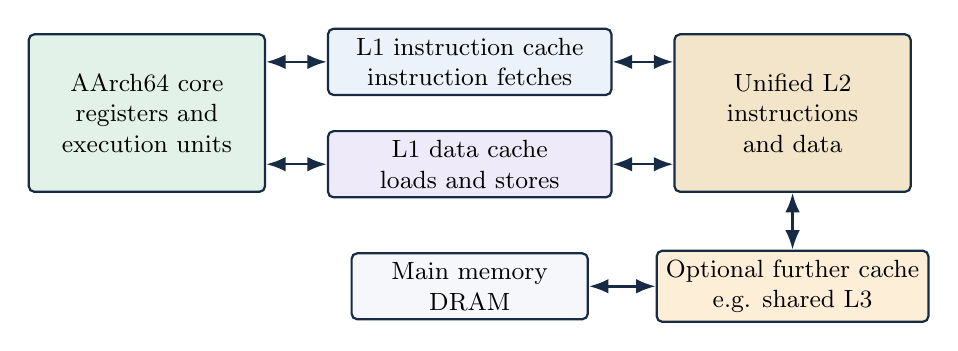
\begin{tikzpicture}[font=\small]
  \node[cachebox,fill=softgreen,minimum width=3cm,minimum height=2cm] (r) at (0,1.7) {AArch64 core\\registers and\\execution units};
  \node[cachebox,fill=lightblue,minimum width=3.6cm] (i) at (4.1,2.35) {L1 instruction cache\\instruction fetches};
  \node[cachebox,fill=softpurple,minimum width=3.6cm] (d) at (4.1,1.05) {L1 data cache\\loads and stores};
  \node[cachebox,fill=gold!24,minimum width=3cm,minimum height=2cm] (l2) at (8.2,1.7) {Unified L2\\instructions\\and data};
  \node[cachebox,fill=softorange,minimum width=3cm] (ll) at (8.2,-.5) {Optional further cache\\e.g. shared L3};
  \node[cachebox,fill=softgray,minimum width=3cm] (ram) at (4.1,-.5) {Main memory\\DRAM};
  \draw[twoway] (r.east|-i.west)--(i.west);
  \draw[twoway] (r.east|-d.west)--(d.west);
  \draw[twoway] (i.east)--(i.east-|l2.west);
  \draw[twoway] (d.east)--(d.east-|l2.west);
  \draw[twoway] (l2.south)--(ll.north);
  \draw[twoway] (ll.west)--(ram.east);
\end{tikzpicture}
\end{center}
\begin{itemize}\setlength{\itemsep}{4pt}
  \item Typical organization: separate L1 instruction/data caches; unified lower levels. Sizes, sharing, and levels vary by implementation.
  \item Caches commonly use SRAM (static RAM); main memory uses denser DRAM (dynamic RAM).
  \item SSD/disk storage is accessed through software and I/O. A normal cache miss does not directly fetch a line from disk.
\end{itemize}
\end{frame}

% CONTENT 04
\begin{frame}{A Cache Line Contains Neighbouring Bytes}
\small
\Model{64-byte lines; cacheable Normal memory; valid aligned load; \code{x0=0x1000}; line initially absent.}
\code{ldr x2, [x0, \#16]} requests bytes \hex{1010}--\hex{1017}.
\begin{center}
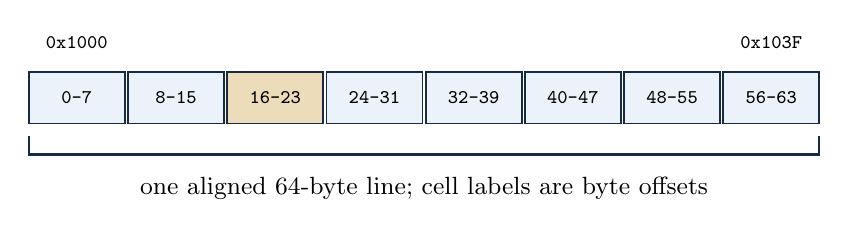
\begin{tikzpicture}
  \EightWords{lightblue}
  \node[memcell,fill=gold!32] at (2.52,0) {16-23};
  \node[font=\ttfamily\scriptsize,above] at (0,.5) {0x1000};
  \node[font=\ttfamily\scriptsize,above] at (8.82,.5) {0x103F};
  \draw[draw=navy,line width=.8pt]
    (-.61,-.48)--(-.61,-.72)--(9.43,-.72)--(9.43,-.48);
  \node[font=\small,anchor=north] at (4.41,-.88)
    {one aligned 64-byte line; cell labels are byte offsets};
\end{tikzpicture}
\end{center}
\begin{itemize}\setlength{\itemsep}{4pt}
  \item \key{Access width: 8 bytes. Line-fill size: 64 bytes.} The cache fetches the line at \hex{1000}.
  \item A 64-byte line holds eight 64-bit values, sixteen 32-bit values, or sixteen 4-byte A64 instructions.
  \item Neighbouring accesses can reuse the fetched line while it remains resident.
  \item Line base \(=\lfloor\text{address}/64\rfloor\times64\). A line boundary is independent of source-level object boundaries.
\end{itemize}
\end{frame}

% CONTENT 05
\begin{frame}{Temporal and Spatial Locality}
\begin{columns}[T,onlytextwidth]
\column{.48\textwidth}
\begin{block}{Temporal: reuse loop instructions}
\Asm{mov  x1, \#8\\.Lloop:\\subs x1, x1, \#1\\b.ne .Lloop}
\end{block}
\small
Each iteration reuses the same \code{subs} and \code{b.ne} instructions: temporal locality in instruction fetch.
\column{.48\textwidth}
\begin{block}{Spatial: access nearby locations}
\Asm{ldr x2, [x0]\\ldr x3, [x0, \#8]}
\end{block}
\small
With \code{x0} aligned to a 64-byte line, both loads use the same line. The first fill supplies the second value too.
\end{columns}
\vspace{.25cm}
\begin{itemize}\setlength{\itemsep}{6pt}
  \item Caching recently used lines exploits temporal locality; fetching neighbouring bytes exploits spatial locality.
  \item Repeated accesses to the same memory variable can also have temporal locality.
  \item Reusing a value already held in an X register creates no new data-cache access.
\end{itemize}
\end{frame}

% CONTENT 06
\begin{frame}{Sequential AArch64 Loads Reuse One Line}
\small
\Model{Cold cache; 64-byte lines; aligned base \hex{1000}; eight 64-bit values; no prefetching.}
\begin{columns}[T,onlytextwidth]
\column{.42\textwidth}
\begin{block}{Pointer advances by eight bytes}
\Asm{.Lsum:\\ldr  x2, [x0], \#8\\add  x3, x3, x2\\subs x1, x1, \#1\\b.ne .Lsum}
\end{block}
\small Initially \code{x1=8}, \code{x3=0}. Post-indexing uses the old \code{x0}, then adds 8.
\column{.54\textwidth}
\renewcommand{\arraystretch}{1.3}
\begin{tabular}{R{2.7cm}R{3.7cm}}
\toprule
\textbf{Load address} & \textbf{Data-cache result}\\
\midrule
\hex{1000} & miss; fetch the line\\
\hex{1008}--\hex{1038}\newline in steps of 8 & seven hits in that line\\
\bottomrule
\end{tabular}\par
\vspace{.2cm}
Eight data loads: \key{one miss, seven hits}. Miss rate \(=1/8=12.5\%\).
\end{columns}
\vspace{.2cm}
\small The loop's instruction fetches are separate cache references. The count above describes only its eight data loads.
\end{frame}

% CONTENT 07
\begin{frame}{Stride Determines How Much of Each Line Is Used}
\small
\Model{Eight 8-byte loads; cold cache; base \hex{1000}; 64-byte lines; enough capacity; no prefetching.}
\renewcommand{\arraystretch}{1.4}
\setlength{\tabcolsep}{4pt}
\begin{tabular}{R{2.9cm}R{4.4cm}R{2.3cm}R{2.9cm}}
\toprule
\textbf{Address stride} & \textbf{Load addresses} & \textbf{Lines fetched} & \textbf{Useful bytes / fetched bytes}\\
\midrule
8 bytes & \hex{1000}, \hex{1008}, \ldots, \hex{1038} & 1 & \(64/64=100\%\)\\
64 bytes & \hex{1000}, \hex{1040}, \ldots, \hex{11C0} & 8 & \(64/512=12.5\%\)\\
\bottomrule
\end{tabular}\par
\vspace{.23cm}
\begin{itemize}\setlength{\itemsep}{6pt}
  \item Both sequences request 64 useful bytes. The second transfers eight times as many line-fill bytes.
  \item The \key{working set} is the collection of lines needed over a period of execution.
  \item Reuse depends on whether that working set remains resident: total capacity, set placement, and replacement all matter.
\end{itemize}
\end{frame}

\sectiondivider{PART 2}{Cache Organization and Address Mapping}

% CONTENT 08
\begin{frame}{Capacity, Line Size, Sets, and Ways}
\small
\begin{block}{Cache data capacity}
\[
C=S\times A\times B
\qquad\Longrightarrow\qquad
S=\frac{C}{A B}
\]
\end{block}
\renewcommand{\arraystretch}{1.3}
\begin{tabular}{R{3.0cm}R{5.3cm}R{4.8cm}}
\toprule
\textbf{Parameter} & \textbf{Meaning} & \textbf{Main worked configuration}\\
\midrule
\(C\): capacity & data bytes stored; metadata excluded & 32 KiB \(=32{,}768\) bytes\\
\(B\): line size & bytes in one line & 64 bytes\\
\(A\): associativity & lines (ways) in each set & 4 ways\\
\(S\): set count & independently indexed sets & \(32{,}768/(4\times64)=128\)\\
\bottomrule
\end{tabular}\par
\vspace{.18cm}
This cache holds \(128\times4=512\) lines. Each memory line has one candidate set and can occupy any of its four ways.
\SourceNote{Mapping example: 48-bit physical addresses; assume identity translation and ordinary low-bit indexing. No prefetching or other-core traffic. Smaller caches are labelled separately.}
\end{frame}

% CONTENT 09
\begin{frame}{Split the Address into Tag, Set Index, and Offset}
\small
\Model{Byte address \(a\); 48-bit physical addresses; 32 KiB data; 4 ways; 64-byte lines; 128 sets.}
\begin{center}
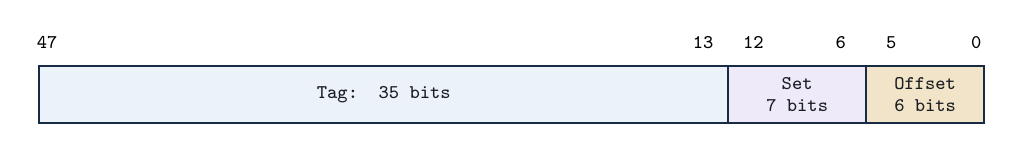
\begin{tikzpicture}
  \bfld{0}{0}{8.75}{Tag: 35 bits}{lightblue}
  \bfld{8.75}{0}{1.75}{Set\\7 bits}{softpurple}
  \bfld{10.5}{0}{1.5}{Offset\\6 bits}{gold!25}
  \node[font=\ttfamily\scriptsize,above] at (.1,.82) {47};
  \node[font=\ttfamily\scriptsize,above] at (8.43,.82) {13};
  \node[font=\ttfamily\scriptsize,above] at (9.07,.82) {12};
  \node[font=\ttfamily\scriptsize,above] at (10.18,.82) {6};
  \node[font=\ttfamily\scriptsize,above] at (10.82,.82) {5};
  \node[font=\ttfamily\scriptsize,above] at (11.9,.82) {0};
\end{tikzpicture}
\end{center}
\[
\text{line number}=\left\lfloor\frac{a}{64}\right\rfloor,\quad
\text{set}=\text{line number}\bmod128,\quad
\text{tag}=\left\lfloor\frac{\text{line number}}{128}\right\rfloor
\]
\begin{itemize}\setlength{\itemsep}{5pt}
  \item The offset selects a byte within a line; the index selects a set; the tag identifies which memory line occupies a way.
  \item Address \hex{1238}: line number 72, set 72 (\hex{48}), tag 0, byte offset 56 (\hex{38}).
  \item \code{ldr x2, [x0]} with \code{x0=0x1238} reads the last eight bytes of the line at \hex{1200}.
\end{itemize}
\SourceNote{The 48-bit width is an example physical-address width. An AArch64 X address register remains 64 bits wide.}
\end{frame}

% CONTENT 10
\begin{frame}{Direct Mapping: One Possible Cache Location}
\small
\Model{Small example: 256-byte data cache; four 64-byte lines; one way per set.}
\begin{center}
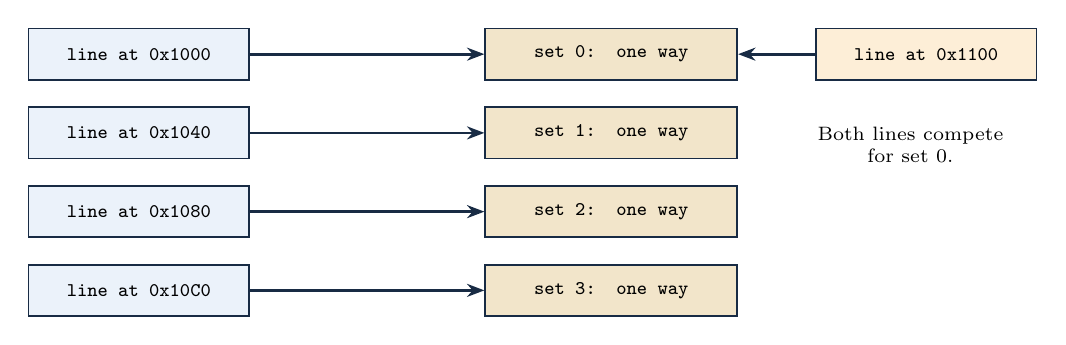
\begin{tikzpicture}[font=\small]
  \foreach \y/\addr/\idx in {1.5/1000/0,.5/1040/1,-.5/1080/2,-1.5/10C0/3} {
    \node[memcell,fill=lightblue,minimum width=2.8cm] (m\idx) at (0,\y) {line at 0x\addr};
    \node[memcell,fill=gold!24,minimum width=3.2cm] (c\idx) at (6,\y) {set \idx: one way};
    \draw[bus] (m\idx.east)--(c\idx.west);
  }
  \node[memcell,fill=softorange,minimum width=2.8cm] (other) at (10,1.5) {line at 0x1100};
  \draw[bus] (other.west)--(c0.east);
  \node[font=\scriptsize,align=center] at (9.8,.35) {Both lines compete\\for set 0.};
\end{tikzpicture}
\end{center}
\begin{itemize}\setlength{\itemsep}{4pt}
  \item Set index \(=\lfloor a/64\rfloor\bmod4\). Addresses separated by 256 bytes have the same index.
  \item A valid line with a matching tag gives a \key{hit}; otherwise the access is a \key{miss}.
  \item Set 0 cannot hold the lines at \hex{1000} and \hex{1100} simultaneously, even when other sets are empty.
\end{itemize}
\end{frame}

% CONTENT 11
\begin{frame}{A Direct-Mapped Trace: Hit, Then Conflict}
\small
\Model{256-byte direct-mapped cache; 64-byte lines; initially all valid bits are 0.}
Each address below is used by \code{ldr x2, [x0]}.
\vspace{.16cm}
\renewcommand{\arraystretch}{1.4}
\setlength{\tabcolsep}{4pt}
\begin{tabular}{R{2.3cm}R{1.4cm}R{1.5cm}R{2.1cm}R{5.0cm}}
\toprule
\textbf{Address} & \textbf{Set} & \textbf{Tag} & \textbf{Result} & \textbf{Set 0 after access}\\
\midrule
\hex{1000} & 0 & 16 & miss & valid; line at \hex{1000}\\
\hex{1008} & 0 & 16 & hit & same line; different offset\\
\hex{1100} & 0 & 17 & miss & replace with line at \hex{1100}\\
\hex{1000} & 0 & 16 & miss & replace with line at \hex{1000}\\
\bottomrule
\end{tabular}\par
\vspace{.22cm}
\begin{itemize}\setlength{\itemsep}{5pt}
  \item First access to each distinct line is compulsory. The final miss is a conflict miss: two lines fit in total capacity but collide in one set.
  \item Hit rate \(=1/4=25\%\); miss rate \(=3/4=75\%\).
  \item Compare tags only when the valid bit is set. An uninitialized tag value cannot create a hit.
\end{itemize}
\end{frame}

% CONTENT 12
\begin{frame}{Associativity Gives a Line More Candidate Locations}
\small
\Model{Hold capacity at 256 bytes and line size at 64 bytes.}
\renewcommand{\arraystretch}{1.4}
\setlength{\tabcolsep}{4pt}
\begin{tabular}{R{4.0cm}R{1.8cm}R{2.4cm}R{4.3cm}}
\toprule
\textbf{Organization} & \textbf{Sets} & \textbf{Ways per set} & \textbf{Candidate locations}\\
\midrule
Direct mapped & 4 & 1 & one line in one selected set\\
2-way set associative & 2 & 2 & either way in one selected set\\
Fully associative & 1 & 4 & any of the four lines\\
\bottomrule
\end{tabular}\par
\vspace{.22cm}
\begin{center}
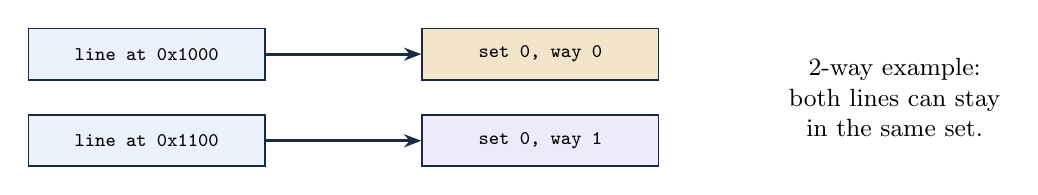
\begin{tikzpicture}[font=\small]
  \node[memcell,fill=lightblue,minimum width=3cm] (a) at (0,.55) {line at 0x1000};
  \node[memcell,fill=lightblue,minimum width=3cm] (b) at (0,-.55) {line at 0x1100};
  \node[memcell,fill=gold!24,minimum width=3cm] (w0) at (5,.55) {set 0, way 0};
  \node[memcell,fill=softpurple,minimum width=3cm] (w1) at (5,-.55) {set 0, way 1};
  \draw[bus] (a.east)--(w0.west);
  \draw[bus] (b.east)--(w1.west);
  \node[align=center,font=\small] at (9.5,0) {2-way example:\\both lines can stay\\in the same set.};
\end{tikzpicture}
\end{center}
\small More ways reduce placement restrictions, but require more tag comparisons and data selection hardware.
\end{frame}

% CONTENT 13
\begin{frame}{Cache Lookup: Select a Set, Compare Tags, Select Data}
\small
\Model{Conceptual 2-way lookup; the offset selects bytes within the matching line.}
\begin{center}
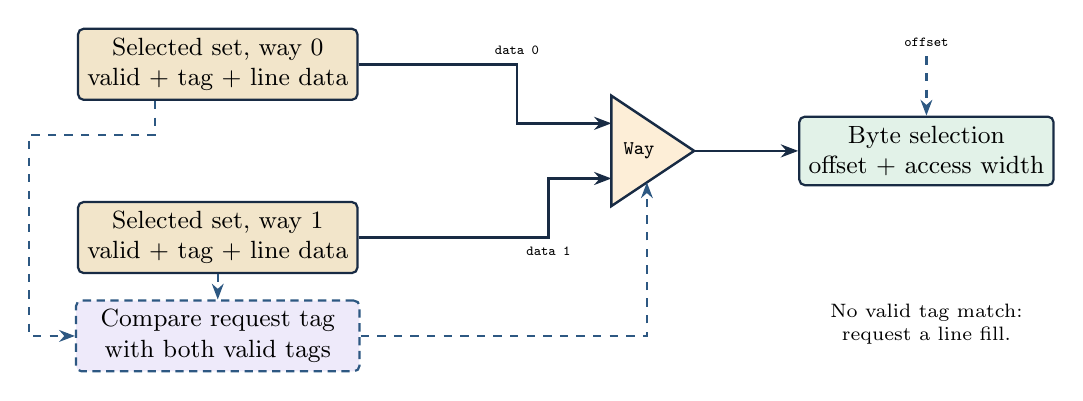
\begin{tikzpicture}[font=\scriptsize]
  \node[state,minimum width=3.5cm,minimum height=.8cm] (w0) at (1,1.1) {Selected set, way 0\\valid + tag + line data};
  \node[state,minimum width=3.5cm,minimum height=.8cm] (w1) at (1,-1.1) {Selected set, way 1\\valid + tag + line data};
  \node[controlunit,minimum width=3.6cm,minimum height=.8cm] (match) at (1,-2.35) {Compare request tag\\with both valid tags};
  \pic (mux) at (6,0) {muxright={Way}};
  \node[logic,minimum width=2.6cm,minimum height=.85cm] (bytes) at (10,0) {Byte selection\\offset + access width};
  \draw[bus] (w0.east)--(4.8,1.1)--(4.8,.35)--(mux-upper);
  \draw[bus] (w1.east)--(5.2,-1.1)--(5.2,-.35)--(mux-lower);
  \draw[bus] (mux-out)--(bytes.west);
  \draw[ctrl] ([xshift=-.8cm]w0.south)--(.2,.2)--(-1.4,.2)--(-1.4,-2.35)--(match.west);
  \draw[ctrl] (w1.south)--(match.north);
  \draw[ctrl] (match.east)--(6.45,-2.35)--(mux-selS);
  \draw[ctrl] (10,1.2)--(bytes.north);
  \node[font=\ttfamily\tiny,above] at (10,1.2) {offset};
  \node[font=\ttfamily\tiny,above] at (4.8,1.1) {data 0};
  \node[font=\ttfamily\tiny,below] at (5.2,-1.1) {data 1};
  \node[font=\scriptsize,align=center] at (10,-2.2) {No valid tag match:\\request a line fill.};
\end{tikzpicture}
\end{center}
\begin{itemize}\setlength{\itemsep}{4pt}
  \item \code{Hit = (V0 \& tag0==requestTag) | (V1 \& tag1==requestTag)}.
  \item The triangle selects the matching way's data; tags distinguish lines sharing a set.
\end{itemize}
\end{frame}

% CONTENT 14
\begin{frame}{Replacement: Choose an Invalid Way, Then a Victim}
\small
\Model{256-byte cache; two sets; two ways; 64-byte lines; LRU replacement; initially empty.}
\key{Victim}: a resident cache line selected for eviction.\par
\key{LRU}: least recently used. A hit makes its line most recently used.
\vspace{.17cm}
\renewcommand{\arraystretch}{1.15}
\setlength{\tabcolsep}{4pt}
\begin{tabular}{R{2.4cm}R{1.6cm}R{3.9cm}R{4.4cm}}
\toprule
\textbf{Load address} & \textbf{Result} & \textbf{Set 0 contents} & \textbf{Action}\\
\midrule
\hex{1000} & miss & \hex{1000}, empty & use an invalid way\\
\hex{1080} & miss & \hex{1000}, \hex{1080} & use the other invalid way\\
\hex{1000} & hit & \hex{1000}, \hex{1080} & \hex{1080} is now LRU\\
\hex{1100} & miss & \hex{1000}, \hex{1100} & evict \hex{1080}\\
\hex{1080} & miss & \hex{1080}, \hex{1100} & evict \hex{1000}\\
\bottomrule
\end{tabular}\par
\vspace{.2cm}
\begin{itemize}\setlength{\itemsep}{5pt}
  \item All three lines compete for two ways in set 0; set 1 remains unused.
  \item Placement chooses the set; replacement chooses the line that leaves.
  \item These traces use LRU. AArch64 does not mandate a replacement algorithm.
\end{itemize}
\end{frame}

% CONTENT 15
\begin{frame}{Why Did the Access Miss? The Three Cs}
\small
\renewcommand{\arraystretch}{1.18}
\begin{tabular}{R{2.7cm}R{5.8cm}R{4.5cm}}
\toprule
\textbf{Miss class} & \textbf{Cause} & \textbf{Possible improvement}\\
\midrule
Compulsory & First reference to a line in an initially cold cache. & Use more bytes from each fetched line; prefetch may hide its latency.\\
Capacity & Reuse fails even in a same-capacity fully associative LRU cache. & Reduce the active working set or increase capacity.\\
Conflict & Reuse fails here, but would hit in that fully associative LRU cache. & Increase associativity or change the address layout.\\
\bottomrule
\end{tabular}\par
\vspace{.22cm}
\begin{itemize}\setlength{\itemsep}{4pt}
  \item Classify first references as compulsory before considering capacity or conflict.
  \item The trace and cache organization together determine the miss rate.
  \item Coherence invalidations can cause additional misses; they are outside these traces.
\end{itemize}
\end{frame}

% CONTENT 16
\begin{frame}{A Small Working Set Can Still Thrash One Set}
\small
\Model{Main cache: 32 KiB, 4 ways, 64-byte lines, 128 sets, LRU. Repeat the five loads below.}
\begin{center}
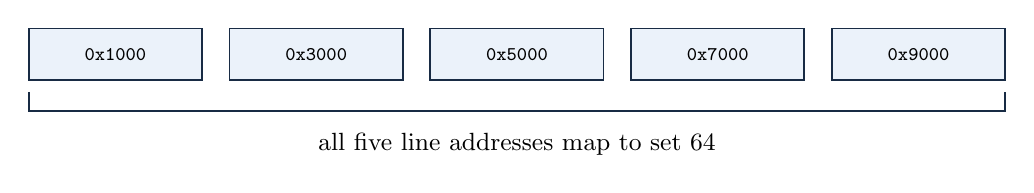
\begin{tikzpicture}
  \foreach \x/\addr in {0/1000,2.55/3000,5.1/5000,7.65/7000,10.2/9000} {
    \node[memcell,fill=lightblue,minimum width=2.2cm] at (\x,0) {0x\addr};
  }
  \draw[draw=navy,line width=.8pt]
    (-1.1,-.48)--(-1.1,-.72)--(11.3,-.72)--(11.3,-.48);
  \node[font=\small,anchor=north] at (5.1,-.88)
    {all five line addresses map to set 64};
\end{tikzpicture}
\end{center}
\begin{itemize}\setlength{\itemsep}{6pt}
  \item Address spacing is \hex{2000} \(=8192=128\times64\) bytes: identical set index, different tags.
  \item Only \(5\times64=320\) data bytes are needed, but that set has four ways. Every access misses during the repeated round-robin trace.
  \item After the compulsory misses, these are \key{conflict misses}: a 512-line fully associative cache would retain all five lines.
  \item By contrast, repeatedly scanning 40 KiB of distinct lines exceeds the 32 KiB capacity; a fully associative LRU cache also misses on the next scan.
\end{itemize}
\end{frame}

\sectiondivider{PART 3}{Stores and Cache Performance}

% CONTENT 17
\begin{frame}{A Read Miss Fetches a Line from the Next Level}
\small
\Model{Blocking cache; read allocation; 64-byte lines; valid memory translation; no prefetching.}
\begin{center}
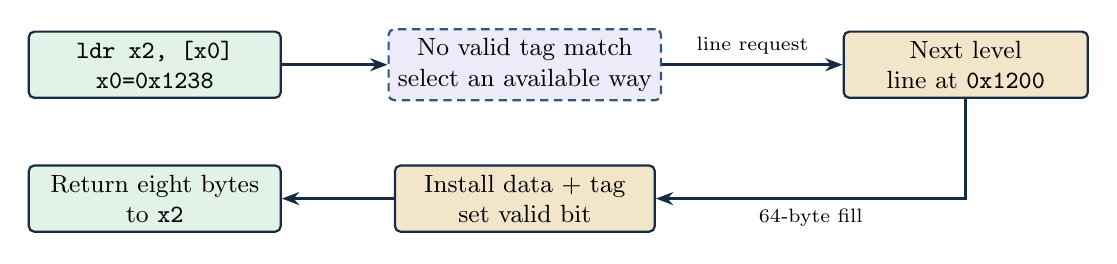
\begin{tikzpicture}[font=\small]
  \node[logic,minimum width=3.2cm] (load) at (0,1.0) {\code{ldr x2, [x0]}\\\code{x0=0x1238}};
  \node[controlunit,minimum width=3.3cm] (miss) at (4.7,1.0) {No valid tag match\\select an available way};
  \node[state,minimum width=3.1cm] (lower) at (10.3,1.0) {Next level\\line at \hex{1200}};
  \node[state,minimum width=3.3cm] (fill) at (4.7,-.7) {Install data + tag\\set valid bit};
  \node[logic,minimum width=3.2cm] (reg) at (0,-.7) {Return eight bytes\\to \code{x2}};
  \draw[bus] (load.east)--(miss.west);
  \draw[bus] (miss.east)--node[above,font=\scriptsize]{line request}(lower.west);
  \draw[bus] (lower.south)--(10.3,-.7)--node[below,font=\scriptsize]{64-byte fill}(fill.east);
  \draw[bus] (fill.west)--(reg.east);
\end{tikzpicture}
\end{center}
\begin{itemize}\setlength{\itemsep}{5pt}
  \item The next level can be L2, another cache, or DRAM; an L1 miss need not reach DRAM.
  \item Before evicting a line with pending writes (a \key{dirty victim}), write it back. Clean or invalid lines need no data writeback.
  \item Return bytes \hex{1238}--\hex{123F} from the fetched line at \hex{1200}.
  \item A cache miss changes timing; it does not itself imply a page fault.
\end{itemize}
\end{frame}

% CONTENT 18
\begin{frame}{Store Hits: Write-Through or Write-Back}
\small
\Model{\code{str x2, [x0, \#8]}; \code{x0=0x1000}; the 64-byte line is already present.}
\begin{center}
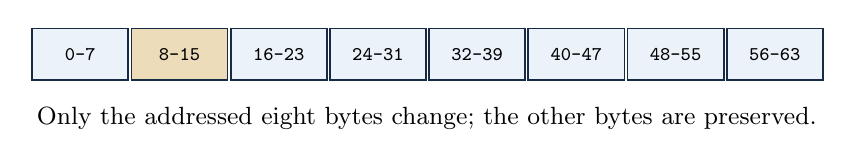
\begin{tikzpicture}
  \EightWords{lightblue}
  \node[memcell,fill=gold!32] at (1.26,0) {8-15};
  \node[font=\small,below] at (4.4,-.55) {Only the addressed eight bytes change; the other bytes are preserved.};
\end{tikzpicture}
\end{center}
\renewcommand{\arraystretch}{1.35}
\begin{tabular}{R{3.0cm}R{5.1cm}R{4.9cm}}
\toprule
\textbf{Hit policy} & \textbf{Action} & \textbf{Consequence}\\
\midrule
Write-through & Update the cached bytes and send the write to the next level. & More outgoing write traffic; buffering can decouple the core from it.\\
Write-back & Update the cached bytes and set a dirty bit. & The newest bytes may exist only in this cache until writeback.\\
\bottomrule
\end{tabular}\par
\vspace{.18cm}
\small A \key{dirty} line may differ from the next level's copy. Eviction requires writeback; maintenance or coherence may also cause writeback in real systems.
\end{frame}

% CONTENT 19
\begin{frame}{Store Misses: Allocate a Line or Bypass This Cache}
\small
\code{str x2, [x0]} targets a line that is absent.
\begin{columns}[T,onlytextwidth]
\column{.48\textwidth}
\begin{block}{Write allocate}
\begin{enumerate}\setlength{\itemsep}{5pt}
  \item Obtain the line from the next level.
  \item Install it in this cache.
  \item Update the store's bytes.
\end{enumerate}
\end{block}
\small With write-back, mark the installed line dirty. A later access can hit while it remains resident.
\column{.48\textwidth}
\begin{block}{No write allocate}
\begin{enumerate}\setlength{\itemsep}{5pt}
  \item Send the write to the next level.
  \item Do not install the missed line in this cache.
\end{enumerate}
\end{block}
\small A later load must obtain the line if it is still absent. The next level follows its own policy.
\end{columns}
\vspace{.24cm}
\begin{itemize}\setlength{\itemsep}{6pt}
  \item Write-through/write-back describes \key{write hits}; allocation describes \key{write misses}. They are separate choices.
  \item Worked store traces use \key{write-back + write allocate}, with full-line fills and writebacks. Optimized full-line stores are outside this model.
\end{itemize}
\end{frame}

% CONTENT 20
\begin{frame}{Dirty Eviction Uses the Victim's Address}
\small
\Model{256-byte direct-mapped cache; 64-byte lines; write-back. Set 0 holds dirty line \hex{1000}.}
A load at \hex{1100} needs the same set. The old line's tag is 16; the new tag is 17.
\begin{center}
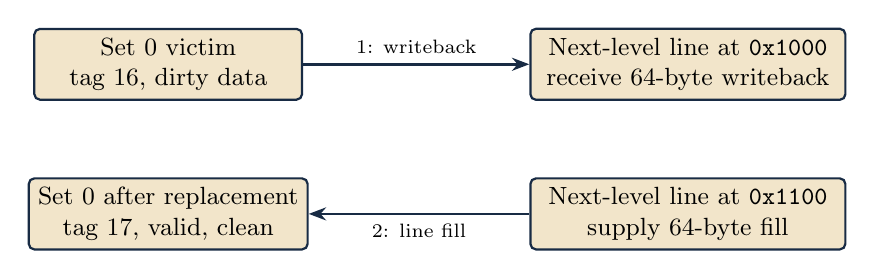
\begin{tikzpicture}[font=\small]
  \node[state,minimum width=3.4cm] (victim) at (0,1) {Set 0 victim\\tag 16, dirty data};
  \node[state,minimum width=4.0cm] (old) at (6.6,1) {Next-level line at \hex{1000}\\receive 64-byte writeback};
  \node[state,minimum width=4.0cm] (new) at (6.6,-.9) {Next-level line at \hex{1100}\\supply 64-byte fill};
  \node[state,minimum width=3.4cm] (installed) at (0,-.9) {Set 0 after replacement\\tag 17, valid, clean};
  \draw[bus] (victim.east)--node[above,font=\scriptsize]{1: writeback}(old.west);
  \draw[bus] (new.west)--node[below,font=\scriptsize]{2: line fill}(installed.east);
\end{tikzpicture}
\end{center}
\begin{itemize}\setlength{\itemsep}{5pt}
  \item Reconstruct the victim line base from \key{its saved tag and set index}: \((16\times4+0)\times64=\hex{1000}\).
  \item Writing dirty data to the new request's address would corrupt a different memory line.
  \item At this cache boundary: clean read miss transfers 64 fill bytes; dirty read miss transfers \(64+64=128\) data bytes. Control traffic is excluded.
\end{itemize}
\end{frame}

% CONTENT 21
\begin{frame}{Average Memory Access Time: Hits and Misses}
\small
Average memory access time (\key{AMAT}) combines the hit cost with the additional miss cost.
\begin{block}{One cache level}
\centering \(\mathrm{AMAT}=t_{\mathrm{hit}}+m\times p_{\mathrm{miss}}\)
\end{block}
\(m\): misses / accesses. \quad \(p_{\mathrm{miss}}\): \key{additional} time after the hit lookup fails.
\par\vspace{.14cm}
One nanosecond (ns) is \(10^{-9}\) seconds. Timings below are illustrative.
\vspace{.17cm}
\renewcommand{\arraystretch}{1.35}
\begin{tabular}{R{7.5cm}R{5.6cm}}
\toprule
\textbf{Configuration} & \textbf{Average}\\
\midrule
Hit time 1 ns; miss rate 5\%; penalty 60 ns & \(1+0.05\times60=4\) ns\\
Same timings; miss rate reduced to 1\% & \(1+0.01\times60=1.6\) ns\\
\bottomrule
\end{tabular}\par
\vspace{.2cm}
\begin{itemize}\setlength{\itemsep}{5pt}
  \item A small fraction of expensive misses can dominate the average.
  \item This serial model excludes overlap and queuing. AMAT is not time per instruction.
\end{itemize}
\end{frame}

% CONTENT 22
\begin{frame}{Two Levels: Local Miss Rate and Global Miss Rate}
\small
\Model{L1 hit time 1 ns; L1 miss rate 5\%; L2 lookup 8 ns; L2 local miss rate 10\%; additional memory cost 60 ns.}
\begin{block}{Only L1 misses consult L2}
\[
\mathrm{AMAT}=t_1+m_1(t_2+m_2p)
=1+0.05(8+0.10\times60)=1.7\ \mathrm{ns}
\]
{\scriptsize \(t_1,t_2\): lookup times; \(m_1,m_2\): local miss rates; \(p\): additional memory cost.}
\end{block}
\begin{center}
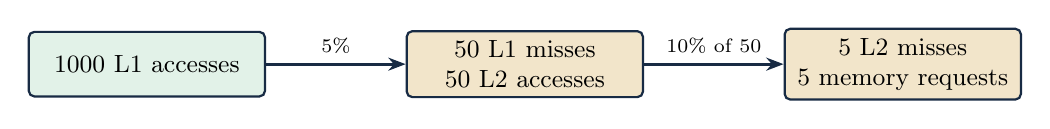
\begin{tikzpicture}[font=\small]
  \node[logic,minimum width=3cm] (all) at (0,0) {1000 L1 accesses};
  \node[state,minimum width=3cm] (l2) at (4.8,0) {50 L1 misses\\50 L2 accesses};
  \node[state,minimum width=3cm] (ram) at (9.6,0) {5 L2 misses\\5 memory requests};
  \draw[bus] (all.east)--node[above,font=\scriptsize]{5\%}(l2.west);
  \draw[bus] (l2.east)--node[above,font=\scriptsize]{10\% of 50}(ram.west);
\end{tikzpicture}
\end{center}
\begin{itemize}\setlength{\itemsep}{5pt}
  \item L2 \key{local} miss rate \(=5/50=10\%\): denominator is L2 accesses.
  \item L2 \key{global} miss rate \(=5/1000=0.5\%=m_1m_2\): denominator is original accesses.
  \item Average extra cost after an L1 miss is \(8+0.10\times60=14\) ns. Do not apply that cost to every L1 hit.
\end{itemize}
\end{frame}

\sectiondivider{PART 4}{AArch64 Program Behaviour}

% CONTENT 23
\begin{frame}{Traversal Order Changes Line Reuse}
\small
\Model{Row-major \(4\times8\) array of 64-bit values; base \hex{4000}; 64-byte rows; cold fully associative 2-line LRU cache; no prefetching.}
\begin{center}
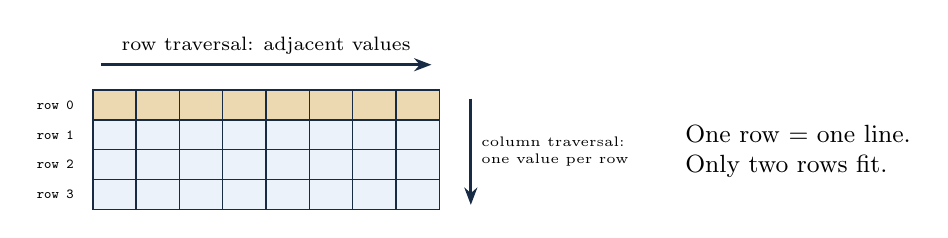
\begin{tikzpicture}[font=\scriptsize]
  \foreach \r in {0,...,3} {
    \foreach \c in {0,...,7} {
      \fill[lightblue] ({.55*\c},{-.38*\r}) rectangle ++(.55,.38);
      \draw[navy,line width=.5pt] ({.55*\c},{-.38*\r}) rectangle ++(.55,.38);
    }
    \node[font=\ttfamily\tiny,anchor=east] at (-.12,{-.38*\r+.19}) {row \r};
  }
  \foreach \c in {0,...,7} {\fill[gold!35] ({.55*\c},0) rectangle ++(.55,.38); \draw[navy,line width=.5pt] ({.55*\c},0) rectangle ++(.55,.38);}
  \draw[bus] (.1,.7)--(4.3,.7) node[midway,above] {row traversal: adjacent values};
  \draw[bus] (4.8,.27)--(4.8,-1.08) node[midway,right,align=left,font=\tiny] {column traversal:\\one value per row};
  \node[font=\small,align=left,anchor=west] at (7.4,-.4) {One row = one line.\\Only two rows fit.};
\end{tikzpicture}
\end{center}
\begin{columns}[T,onlytextwidth]
\column{.48\textwidth}
\begin{block}{Row inner loop: 8-byte stride}
\Asm{ldr x2, [x0]\\add x0, x0, \#8}
\end{block}
\small All 32 loads: \key{4 misses, 28 hits}.
\column{.48\textwidth}
\begin{block}{Column inner loop: 64-byte stride}
\Asm{ldr x2, [x0]\\add x0, x0, \#64}
\end{block}
\small All 32 loads: \key{32 misses, 0 hits}.
\end{columns}
\vspace{.08cm}
\small Outer loops choose row/column starts. If all four lines stay resident, both traversals have four compulsory misses.
\end{frame}

% CONTENT 24
\begin{frame}{Streaming Loads and Dependent Pointer Loads}
\begin{columns}[T,onlytextwidth]
\column{.48\textwidth}
\begin{block}{Contiguous values}
\Asm{ldr x2, [x0]\\ldr x3, [x0, \#8]\\ldr x4, [x0, \#16]}
\end{block}
\small
\begin{itemize}\setlength{\itemsep}{5pt}
  \item Addresses are available from the same base.
  \item Nearby values can share a cache line.
  \item A capable core can overlap independent requests; the ISA does not guarantee this.
\end{itemize}
\column{.48\textwidth}
\begin{block}{Linked nodes; next pointer at offset 0}
\Asm{ldr x0, [x0]\\ldr x0, [x0]\\ldr x0, [x0]}
\end{block}
\small
\begin{itemize}\setlength{\itemsep}{5pt}
  \item Each load supplies the next load's address.
  \item Scattered nodes may have little spatial locality.
  \item The dependency limits overlap along this chain; resident nodes can still hit.
\end{itemize}
\end{columns}
\vspace{.22cm}
\small High bandwidth helps streams of independent transfers. A dependent chain is especially sensitive to access latency.
\end{frame}

% CONTENT 25
\begin{frame}{AArch64 Cache Behaviour and Prefetch Hints}
\small
\begin{block}{Optional software prefetch}
\Asm{prfm pldl1keep, [x0, \#64]\\...\\ldr  x2, [x0, \#64]}
\end{block}
\begin{itemize}\setlength{\itemsep}{4pt}
  \item \code{PLDL1KEEP}: prefetch for a future load, targeting L1 with a temporal retention hint.
  \item \code{prfm} has an implementation-defined effect. It neither loads \code{x2} nor guarantees residency; the \code{ldr} is still required.
  \item Memory attributes make Normal memory cacheable or non-cacheable. Device memory is non-cacheable.
  \item Write policies depend on memory attributes and the processor implementation; \code{ldr}/\code{str} do not select them.
\end{itemize}
\SourceNote{Cache sizes and line lengths vary by implementation; 64-byte lines are examples. Our single-core traces omit translation, coherence, and device ordering.}
\note{Arm PRFM immediate instruction reference: PLD, L1 and KEEP; implementation-defined effect; displayed byte displacement 64 encodes imm12=8. Arm Learn the architecture, Armv8-A memory systems, sections 3 and 4: Normal and Device memory attributes.}
\end{frame}

\begin{frame}{Topic 10 Summary}
\small
\begin{itemize}\setlength{\itemsep}{7pt}
  \item \key{Hierarchy:} smaller, faster levels reduce average access cost; larger levels provide capacity.
  \item \key{Locality:} revisit resident lines and use neighbouring bytes. Access width, line size, stride, and working set are different quantities.
  \item \key{Organization:} capacity \(= \text{sets}\times\text{ways}\times\text{line bytes}\). Index selects a set; valid tag matches identify a hit.
  \item \key{Misses:} distinguish compulsory, capacity, and conflict. More capacity alone does not remove every placement problem.
  \item \key{Stores:} write-hit and write-miss policies are separate; dirty victims must preserve their bytes at the correct next-level address.
  \item \key{Performance:} use consistent AMAT costs and miss-rate denominators. Locality and dependency shape actual program behaviour.
\end{itemize}
\SourceNote{References: \href{https://www.scs.stanford.edu/~zyedidia/arm64/index.html}{Arm-authored A64 instruction specifications};
\href{https://documentation-service.arm.com/static/62d6777531ea212bb6627683}{Arm memory systems};
\href{https://www.cs.cornell.edu/courses/cs3410/2026sp/notes/caches.html}{Cornell cache organization};
\href{https://notes.cs61c.org/content/caches-intro/amat/}{Berkeley AMAT}.}
\end{frame}

\begin{frame}{Self-Test 1: Locality and Address Mapping}
\small
\begin{enumerate}\setlength{\itemsep}{9pt}
  \item Explain why \code{ldr x2, [x0]} reads eight bytes even when a miss fills a 64-byte cache line. How many 64-bit values fit in that line?
  \item From aligned base \hex{2000}, eight loads use an 8-byte stride. Give the addresses, line count, and cold-cache miss rate. Repeat with a 64-byte stride.
  \item A 32 KiB cache has 64-byte lines and four ways. Calculate its line count, set count, and tag/index/offset widths for a 48-bit physical address.
  \item For address \hex{3238} in that cache, calculate the line base, offset, set index, and tag. Why does it share a set with \hex{1238}?
  \item Which locality does repeated instruction fetch in a loop exploit? Why does repeatedly adding to an X-register accumulator create no data-cache references?
\end{enumerate}
\end{frame}

\begin{frame}{Self-Test 2: Mapping, Replacement, and Stores}
\small
\Model{64-byte lines; each trace starts with an empty cache.}
\begin{enumerate}\setlength{\itemsep}{8pt}
  \item Trace loads at \hex{1000}, \hex{1008}, \hex{1100}, \hex{1000} in a 256-byte direct-mapped cache. Give hit/miss outcomes and miss classes.
  \item Repeat with a 256-byte 2-way cache. Explain which outcome changes and why the total data capacity is unchanged.
  \item In that 2-way LRU cache, trace \hex{1000}, \hex{1080}, \hex{1000}, \hex{1100}, \hex{1080}. Identify each victim.
  \item A store misses in a write-back, write-allocate cache. State the line-fill, byte-update, and dirty-bit actions. Contrast no write allocation.
  \item A dirty line at \hex{1000} is replaced by line \hex{1100}. Give the writeback address and data-byte traffic at this boundary, assuming a full 64-byte writeback and fill.
\end{enumerate}
\end{frame}

\begin{frame}{Self-Test 3: Performance and Program Behaviour}
\small
\begin{enumerate}\setlength{\itemsep}{9pt}
  \item Hit time is 2 ns, miss rate 4\%, and additional miss penalty 50 ns. Calculate AMAT. What would it be if the miss rate were 1\%?
  \item L1 hit time is 1 ns and miss rate 8\%; L2 lookup takes 10 ns and its local miss rate is 25\%; memory adds 80 ns. Calculate AMAT and the global L2 miss rate.
  \item Traverse the row-major \(4\times8\) array under the two-line LRU example. Explain the row/column miss counts. What changes if all four rows remain cached?
  \item Why can \code{ldr x0, [x0]} repeated along scattered linked nodes be latency limited even when the memory system supports high bandwidth?
  \item Does \code{prfm pldl1keep, [x0, \#64]} guarantee that a later load hits? Explain why the same cache assumptions cannot be applied to Device memory.
\end{enumerate}
\end{frame}

\end{document}
